\section{GINA- und Rauheitsprotokolle}
\label{sec:anhang_g}
% Inhalt: Messprotokolle der Prüfräder (Auswahl, inventory.md).

Die Messblätter der Verzahnungsmessung und die gedruckten Rauheitsprotokolle der Prüfräder liegen als PDF vor und sind im Inventar der Messungen nach \secref{sec:dokumentation_pruefraeder} gelistet. Als Beispiel folgt das Messblatt der Verzahnungsmessung des Rades 97364 vom 27.05.2026 mit vier Seiten für die Aufspannfehler-Kompensation, das Profil, die Flankenlinie sowie Teilung und Rundlauf. Dazu kommt das Rauheitsprotokoll der linken Flanke desselben Rades. Die Toleranzen auf dem Messblatt sind die der Qualität 7 nach DIN 3962 (\secref{sec:pruefraeder_vorher}).

Die Konturscans der Räder nach dem Lauf sind in \secref{sec:schadensbilder} ausgewertet. \figref{fig:ueberlagerung_97340_z1} zeigt den Zahn 1 des Rades 97340 vor und nach dem Lauf bei $16$\,Nm in derselben Messebene auf dem Sollzahn. Die Abweichung ist nicht überhöht. Die belastete Flanke rechts ist vom Beginn der Verschleißzone bis zum Kopf zurückgesetzt, die unbelastete Flanke links und beide Fußrundungen decken sich mit dem Scan vor dem Lauf.

\begin{figure}[!htbp]
	\centering
	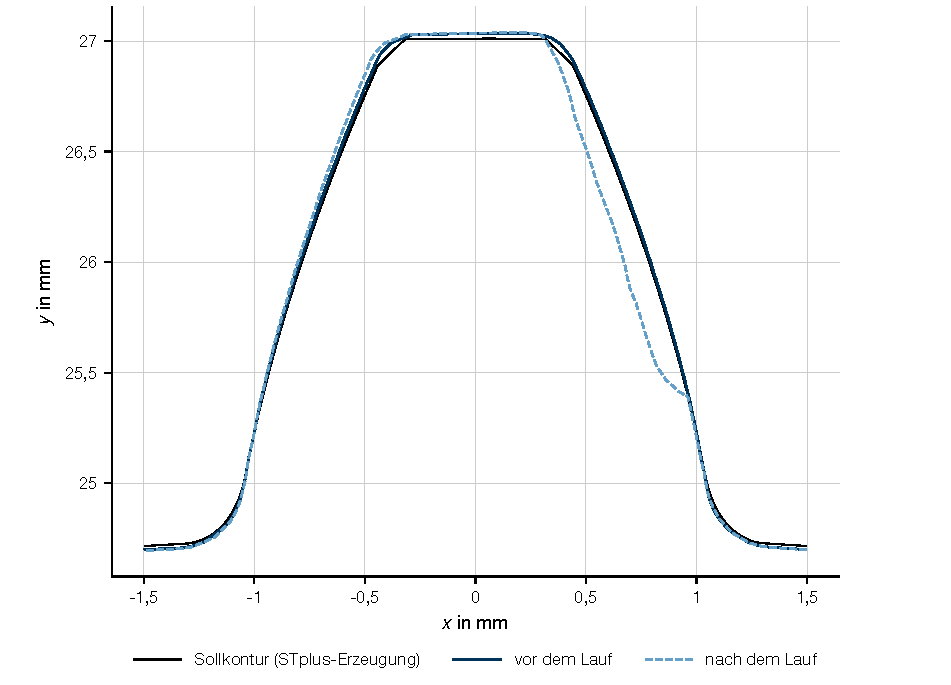
\includegraphics[width=0.8\textwidth]{kap6/ueberlagerung_97340_z1}
	\caption{Zahn 1 des Rades 97340 vor und nach dem Lauf bei $16$\,Nm auf dem Sollzahn der Erzeugung, Messebene $z = 85{,}95$\,mm, Abweichung nicht überhöht.}
	\label{fig:ueberlagerung_97340_z1}
\end{figure}

% Seiten aus 70_input/71_Messungen (Kopien unter bilder/anhang, 2026-10-25): GINA-Messblatt 97364.pdf (4 Seiten), Rauheit 97364-KST_E-li-neu_.pdf.
% Maßstab 0,78 und 4 mm nach unten, damit die Blätter zwischen Kopf- und Fußzeile stehen (Nutzer, 2026-10-26).
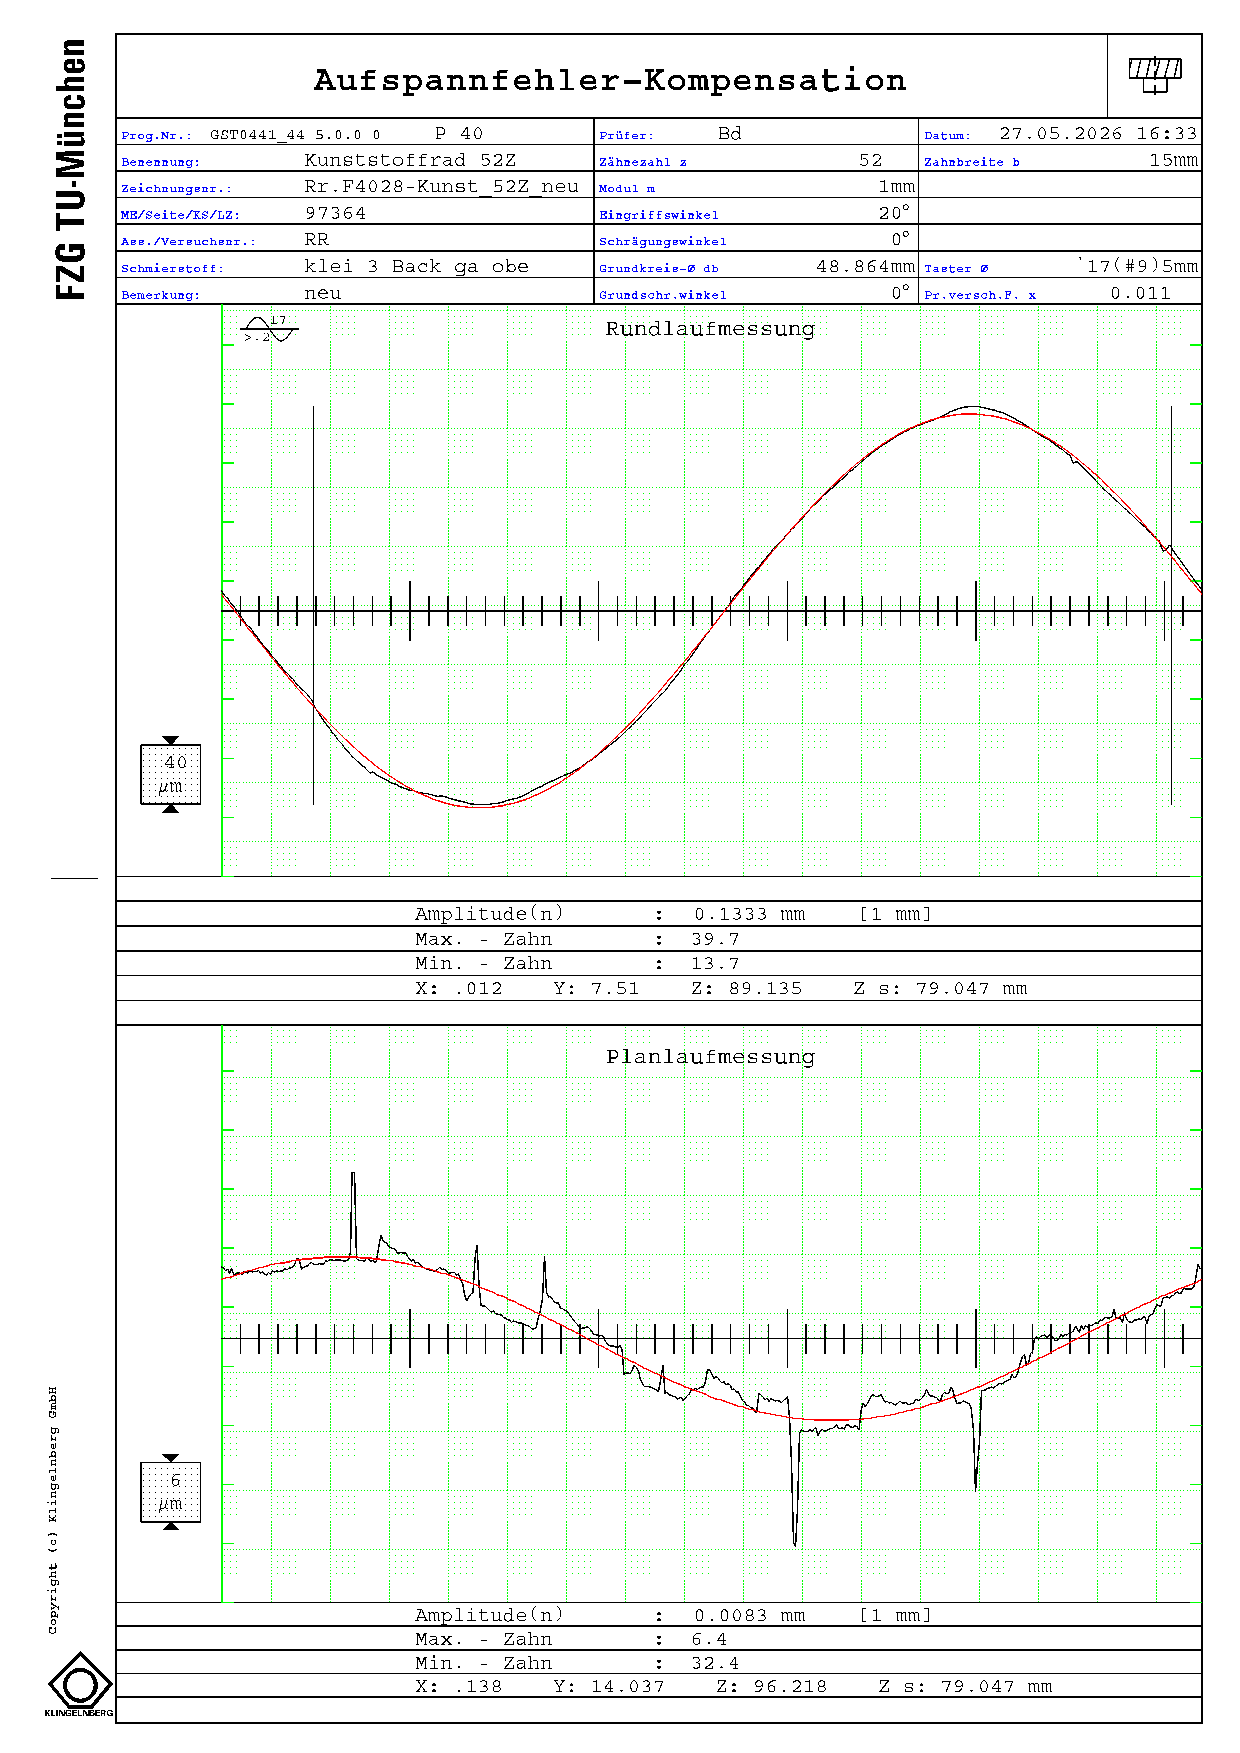
\includepdf[pages=-, scale=0.78, offset=0 -4mm, pagecommand={\thispagestyle{plain}}]{anhang/gina_messblatt_97364.pdf}
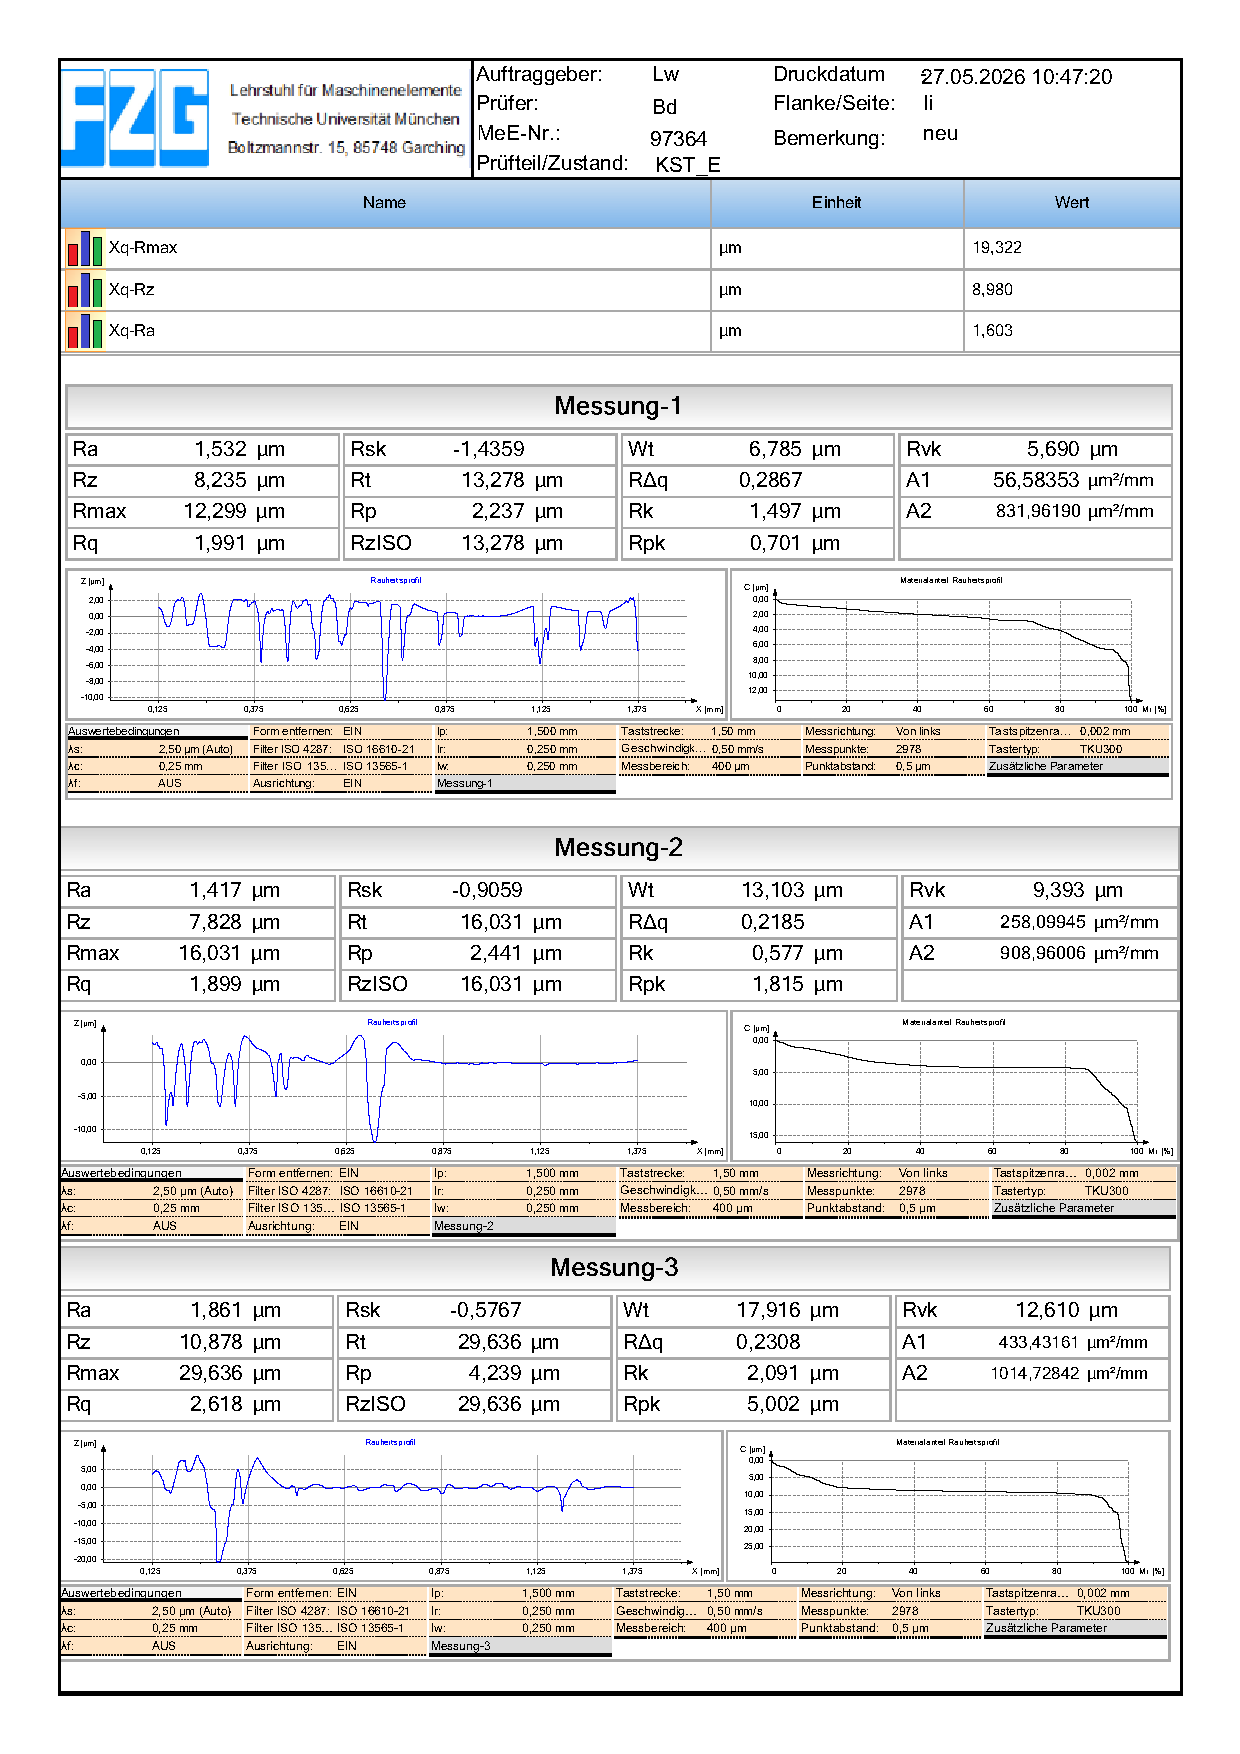
\includepdf[pages=1, scale=0.78, offset=0 -4mm, pagecommand={\thispagestyle{plain}}]{anhang/rauheit_97364_links.pdf}
